% Options for packages loaded elsewhere
\PassOptionsToPackage{unicode}{hyperref}
\PassOptionsToPackage{hyphens}{url}
%
\documentclass[
]{article}
\usepackage{lmodern}
\usepackage{amssymb,amsmath}
\usepackage{ifxetex,ifluatex}
\ifnum 0\ifxetex 1\fi\ifluatex 1\fi=0 % if pdftex
  \usepackage[T1]{fontenc}
  \usepackage[utf8]{inputenc}
  \usepackage{textcomp} % provide euro and other symbols
\else % if luatex or xetex
  \usepackage{unicode-math}
  \defaultfontfeatures{Scale=MatchLowercase}
  \defaultfontfeatures[\rmfamily]{Ligatures=TeX,Scale=1}
\fi
% Use upquote if available, for straight quotes in verbatim environments
\IfFileExists{upquote.sty}{\usepackage{upquote}}{}
\IfFileExists{microtype.sty}{% use microtype if available
  \usepackage[]{microtype}
  \UseMicrotypeSet[protrusion]{basicmath} % disable protrusion for tt fonts
}{}
\makeatletter
\@ifundefined{KOMAClassName}{% if non-KOMA class
  \IfFileExists{parskip.sty}{%
    \usepackage{parskip}
  }{% else
    \setlength{\parindent}{0pt}
    \setlength{\parskip}{6pt plus 2pt minus 1pt}}
}{% if KOMA class
  \KOMAoptions{parskip=half}}
\makeatother
\usepackage{xcolor}
\IfFileExists{xurl.sty}{\usepackage{xurl}}{} % add URL line breaks if available
\IfFileExists{bookmark.sty}{\usepackage{bookmark}}{\usepackage{hyperref}}
\hypersetup{
  pdftitle={Rladies TidyTuesday},
  hidelinks,
  pdfcreator={LaTeX via pandoc}}
\urlstyle{same} % disable monospaced font for URLs
\usepackage[margin=1in]{geometry}
\usepackage{color}
\usepackage{fancyvrb}
\newcommand{\VerbBar}{|}
\newcommand{\VERB}{\Verb[commandchars=\\\{\}]}
\DefineVerbatimEnvironment{Highlighting}{Verbatim}{commandchars=\\\{\}}
% Add ',fontsize=\small' for more characters per line
\usepackage{framed}
\definecolor{shadecolor}{RGB}{248,248,248}
\newenvironment{Shaded}{\begin{snugshade}}{\end{snugshade}}
\newcommand{\AlertTok}[1]{\textcolor[rgb]{0.94,0.16,0.16}{#1}}
\newcommand{\AnnotationTok}[1]{\textcolor[rgb]{0.56,0.35,0.01}{\textbf{\textit{#1}}}}
\newcommand{\AttributeTok}[1]{\textcolor[rgb]{0.77,0.63,0.00}{#1}}
\newcommand{\BaseNTok}[1]{\textcolor[rgb]{0.00,0.00,0.81}{#1}}
\newcommand{\BuiltInTok}[1]{#1}
\newcommand{\CharTok}[1]{\textcolor[rgb]{0.31,0.60,0.02}{#1}}
\newcommand{\CommentTok}[1]{\textcolor[rgb]{0.56,0.35,0.01}{\textit{#1}}}
\newcommand{\CommentVarTok}[1]{\textcolor[rgb]{0.56,0.35,0.01}{\textbf{\textit{#1}}}}
\newcommand{\ConstantTok}[1]{\textcolor[rgb]{0.00,0.00,0.00}{#1}}
\newcommand{\ControlFlowTok}[1]{\textcolor[rgb]{0.13,0.29,0.53}{\textbf{#1}}}
\newcommand{\DataTypeTok}[1]{\textcolor[rgb]{0.13,0.29,0.53}{#1}}
\newcommand{\DecValTok}[1]{\textcolor[rgb]{0.00,0.00,0.81}{#1}}
\newcommand{\DocumentationTok}[1]{\textcolor[rgb]{0.56,0.35,0.01}{\textbf{\textit{#1}}}}
\newcommand{\ErrorTok}[1]{\textcolor[rgb]{0.64,0.00,0.00}{\textbf{#1}}}
\newcommand{\ExtensionTok}[1]{#1}
\newcommand{\FloatTok}[1]{\textcolor[rgb]{0.00,0.00,0.81}{#1}}
\newcommand{\FunctionTok}[1]{\textcolor[rgb]{0.00,0.00,0.00}{#1}}
\newcommand{\ImportTok}[1]{#1}
\newcommand{\InformationTok}[1]{\textcolor[rgb]{0.56,0.35,0.01}{\textbf{\textit{#1}}}}
\newcommand{\KeywordTok}[1]{\textcolor[rgb]{0.13,0.29,0.53}{\textbf{#1}}}
\newcommand{\NormalTok}[1]{#1}
\newcommand{\OperatorTok}[1]{\textcolor[rgb]{0.81,0.36,0.00}{\textbf{#1}}}
\newcommand{\OtherTok}[1]{\textcolor[rgb]{0.56,0.35,0.01}{#1}}
\newcommand{\PreprocessorTok}[1]{\textcolor[rgb]{0.56,0.35,0.01}{\textit{#1}}}
\newcommand{\RegionMarkerTok}[1]{#1}
\newcommand{\SpecialCharTok}[1]{\textcolor[rgb]{0.00,0.00,0.00}{#1}}
\newcommand{\SpecialStringTok}[1]{\textcolor[rgb]{0.31,0.60,0.02}{#1}}
\newcommand{\StringTok}[1]{\textcolor[rgb]{0.31,0.60,0.02}{#1}}
\newcommand{\VariableTok}[1]{\textcolor[rgb]{0.00,0.00,0.00}{#1}}
\newcommand{\VerbatimStringTok}[1]{\textcolor[rgb]{0.31,0.60,0.02}{#1}}
\newcommand{\WarningTok}[1]{\textcolor[rgb]{0.56,0.35,0.01}{\textbf{\textit{#1}}}}
\usepackage{longtable,booktabs}
% Correct order of tables after \paragraph or \subparagraph
\usepackage{etoolbox}
\makeatletter
\patchcmd\longtable{\par}{\if@noskipsec\mbox{}\fi\par}{}{}
\makeatother
% Allow footnotes in longtable head/foot
\IfFileExists{footnotehyper.sty}{\usepackage{footnotehyper}}{\usepackage{footnote}}
\makesavenoteenv{longtable}
\usepackage{graphicx,grffile}
\makeatletter
\def\maxwidth{\ifdim\Gin@nat@width>\linewidth\linewidth\else\Gin@nat@width\fi}
\def\maxheight{\ifdim\Gin@nat@height>\textheight\textheight\else\Gin@nat@height\fi}
\makeatother
% Scale images if necessary, so that they will not overflow the page
% margins by default, and it is still possible to overwrite the defaults
% using explicit options in \includegraphics[width, height, ...]{}
\setkeys{Gin}{width=\maxwidth,height=\maxheight,keepaspectratio}
% Set default figure placement to htbp
\makeatletter
\def\fps@figure{htbp}
\makeatother
\setlength{\emergencystretch}{3em} % prevent overfull lines
\providecommand{\tightlist}{%
  \setlength{\itemsep}{0pt}\setlength{\parskip}{0pt}}
\setcounter{secnumdepth}{-\maxdimen} % remove section numbering

\title{Rladies TidyTuesday}
\author{}
\date{\vspace{-2.5em}26/02/2021}

\begin{document}
\maketitle

\begin{Shaded}
\begin{Highlighting}[]
\NormalTok{tuesdata <-}\StringTok{ }\NormalTok{tidytuesdayR}\OperatorTok{::}\KeywordTok{tt_load}\NormalTok{(}\StringTok{'2021-02-23'}\NormalTok{)}
\end{Highlighting}
\end{Shaded}

\begin{verbatim}
## --- Compiling #TidyTuesday Information for 2021-02-23 ----
\end{verbatim}

\begin{verbatim}
## --- There are 2 files available ---
\end{verbatim}

\begin{verbatim}
## --- Starting Download ---
\end{verbatim}

\begin{verbatim}
## 
##  Downloading file 1 of 2: `earn.csv`
##  Downloading file 2 of 2: `employed.csv`
\end{verbatim}

\begin{verbatim}
## --- Download complete ---
\end{verbatim}

\begin{Shaded}
\begin{Highlighting}[]
\NormalTok{employed <-}\StringTok{ }\NormalTok{tuesdata}\OperatorTok{$}\NormalTok{employed}
\NormalTok{earn <-}\StringTok{ }\NormalTok{readr}\OperatorTok{::}\KeywordTok{read_csv}\NormalTok{(}\StringTok{"https://raw.githubusercontent.com/rfordatascience/tidytuesday/master/data/2021/2021-02-23/earn.csv"}\NormalTok{)}
\end{Highlighting}
\end{Shaded}

\begin{verbatim}
## 
## -- Column specification --------------------------------------------------------
## cols(
##   sex = col_character(),
##   race = col_character(),
##   ethnic_origin = col_character(),
##   age = col_character(),
##   year = col_double(),
##   quarter = col_double(),
##   n_persons = col_double(),
##   median_weekly_earn = col_double()
## )
\end{verbatim}

\begin{Shaded}
\begin{Highlighting}[]
\NormalTok{skimr}\OperatorTok{::}\KeywordTok{skim}\NormalTok{(earn)}
\end{Highlighting}
\end{Shaded}

\begin{longtable}[]{@{}ll@{}}
\caption{Data summary}\tabularnewline
\toprule
\endhead
Name & earn\tabularnewline
Number of rows & 4224\tabularnewline
Number of columns & 8\tabularnewline
\_\_\_\_\_\_\_\_\_\_\_\_\_\_\_\_\_\_\_\_\_\_\_ &\tabularnewline
Column type frequency: &\tabularnewline
character & 4\tabularnewline
numeric & 4\tabularnewline
\_\_\_\_\_\_\_\_\_\_\_\_\_\_\_\_\_\_\_\_\_\_\_\_ &\tabularnewline
Group variables & None\tabularnewline
\bottomrule
\end{longtable}

\textbf{Variable type: character}

\begin{longtable}[]{@{}lrrrrrrr@{}}
\toprule
skim\_variable & n\_missing & complete\_rate & min & max & empty &
n\_unique & whitespace\tabularnewline
\midrule
\endhead
sex & 0 & 1 & 3 & 10 & 0 & 3 & 0\tabularnewline
race & 0 & 1 & 5 & 25 & 0 & 4 & 0\tabularnewline
ethnic\_origin & 0 & 1 & 11 & 18 & 0 & 2 & 0\tabularnewline
age & 0 & 1 & 14 & 17 & 0 & 12 & 0\tabularnewline
\bottomrule
\end{longtable}

\textbf{Variable type: numeric}

\begin{longtable}[]{@{}lrrrrrrrrrl@{}}
\toprule
\begin{minipage}[b]{0.11\columnwidth}\raggedright
skim\_variable\strut
\end{minipage} & \begin{minipage}[b]{0.06\columnwidth}\raggedleft
n\_missing\strut
\end{minipage} & \begin{minipage}[b]{0.08\columnwidth}\raggedleft
complete\_rate\strut
\end{minipage} & \begin{minipage}[b]{0.07\columnwidth}\raggedleft
mean\strut
\end{minipage} & \begin{minipage}[b]{0.07\columnwidth}\raggedleft
sd\strut
\end{minipage} & \begin{minipage}[b]{0.04\columnwidth}\raggedleft
p0\strut
\end{minipage} & \begin{minipage}[b]{0.06\columnwidth}\raggedleft
p25\strut
\end{minipage} & \begin{minipage}[b]{0.06\columnwidth}\raggedleft
p50\strut
\end{minipage} & \begin{minipage}[b]{0.07\columnwidth}\raggedleft
p75\strut
\end{minipage} & \begin{minipage}[b]{0.06\columnwidth}\raggedleft
p100\strut
\end{minipage} & \begin{minipage}[b]{0.04\columnwidth}\raggedright
hist\strut
\end{minipage}\tabularnewline
\midrule
\endhead
\begin{minipage}[t]{0.11\columnwidth}\raggedright
year\strut
\end{minipage} & \begin{minipage}[t]{0.06\columnwidth}\raggedleft
0\strut
\end{minipage} & \begin{minipage}[t]{0.08\columnwidth}\raggedleft
1\strut
\end{minipage} & \begin{minipage}[t]{0.07\columnwidth}\raggedleft
2015.00\strut
\end{minipage} & \begin{minipage}[t]{0.07\columnwidth}\raggedleft
3.16\strut
\end{minipage} & \begin{minipage}[t]{0.04\columnwidth}\raggedleft
2010\strut
\end{minipage} & \begin{minipage}[t]{0.06\columnwidth}\raggedleft
2.012e+03\strut
\end{minipage} & \begin{minipage}[t]{0.06\columnwidth}\raggedleft
2015.0\strut
\end{minipage} & \begin{minipage}[t]{0.07\columnwidth}\raggedleft
2018.00\strut
\end{minipage} & \begin{minipage}[t]{0.06\columnwidth}\raggedleft
2020\strut
\end{minipage} & \begin{minipage}[t]{0.04\columnwidth}\raggedright
▇▅▅▅▅\strut
\end{minipage}\tabularnewline
\begin{minipage}[t]{0.11\columnwidth}\raggedright
quarter\strut
\end{minipage} & \begin{minipage}[t]{0.06\columnwidth}\raggedleft
0\strut
\end{minipage} & \begin{minipage}[t]{0.08\columnwidth}\raggedleft
1\strut
\end{minipage} & \begin{minipage}[t]{0.07\columnwidth}\raggedleft
2.50\strut
\end{minipage} & \begin{minipage}[t]{0.07\columnwidth}\raggedleft
1.12\strut
\end{minipage} & \begin{minipage}[t]{0.04\columnwidth}\raggedleft
1\strut
\end{minipage} & \begin{minipage}[t]{0.06\columnwidth}\raggedleft
1.750e+00\strut
\end{minipage} & \begin{minipage}[t]{0.06\columnwidth}\raggedleft
2.5\strut
\end{minipage} & \begin{minipage}[t]{0.07\columnwidth}\raggedleft
3.25\strut
\end{minipage} & \begin{minipage}[t]{0.06\columnwidth}\raggedleft
4\strut
\end{minipage} & \begin{minipage}[t]{0.04\columnwidth}\raggedright
▇▇▁▇▇\strut
\end{minipage}\tabularnewline
\begin{minipage}[t]{0.11\columnwidth}\raggedright
n\_persons\strut
\end{minipage} & \begin{minipage}[t]{0.06\columnwidth}\raggedleft
0\strut
\end{minipage} & \begin{minipage}[t]{0.08\columnwidth}\raggedleft
1\strut
\end{minipage} & \begin{minipage}[t]{0.07\columnwidth}\raggedleft
16268337.59\strut
\end{minipage} & \begin{minipage}[t]{0.07\columnwidth}\raggedleft
22421840.69\strut
\end{minipage} & \begin{minipage}[t]{0.04\columnwidth}\raggedleft
103000\strut
\end{minipage} & \begin{minipage}[t]{0.06\columnwidth}\raggedleft
2.614e+06\strut
\end{minipage} & \begin{minipage}[t]{0.06\columnwidth}\raggedleft
7441000.0\strut
\end{minipage} & \begin{minipage}[t]{0.07\columnwidth}\raggedleft
17555250.00\strut
\end{minipage} & \begin{minipage}[t]{0.06\columnwidth}\raggedleft
118358000\strut
\end{minipage} & \begin{minipage}[t]{0.04\columnwidth}\raggedright
▇▁▁▁▁\strut
\end{minipage}\tabularnewline
\begin{minipage}[t]{0.11\columnwidth}\raggedright
median\_weekly\_earn\strut
\end{minipage} & \begin{minipage}[t]{0.06\columnwidth}\raggedleft
0\strut
\end{minipage} & \begin{minipage}[t]{0.08\columnwidth}\raggedleft
1\strut
\end{minipage} & \begin{minipage}[t]{0.07\columnwidth}\raggedleft
762.18\strut
\end{minipage} & \begin{minipage}[t]{0.07\columnwidth}\raggedleft
217.21\strut
\end{minipage} & \begin{minipage}[t]{0.04\columnwidth}\raggedleft
318\strut
\end{minipage} & \begin{minipage}[t]{0.06\columnwidth}\raggedleft
6.050e+02\strut
\end{minipage} & \begin{minipage}[t]{0.06\columnwidth}\raggedleft
755.0\strut
\end{minipage} & \begin{minipage}[t]{0.07\columnwidth}\raggedleft
911.00\strut
\end{minipage} & \begin{minipage}[t]{0.06\columnwidth}\raggedleft
1709\strut
\end{minipage} & \begin{minipage}[t]{0.04\columnwidth}\raggedright
▅▇▅▁▁\strut
\end{minipage}\tabularnewline
\bottomrule
\end{longtable}

\begin{Shaded}
\begin{Highlighting}[]
\NormalTok{visdat}\OperatorTok{::}\KeywordTok{vis_dat}\NormalTok{(earn)}
\end{Highlighting}
\end{Shaded}

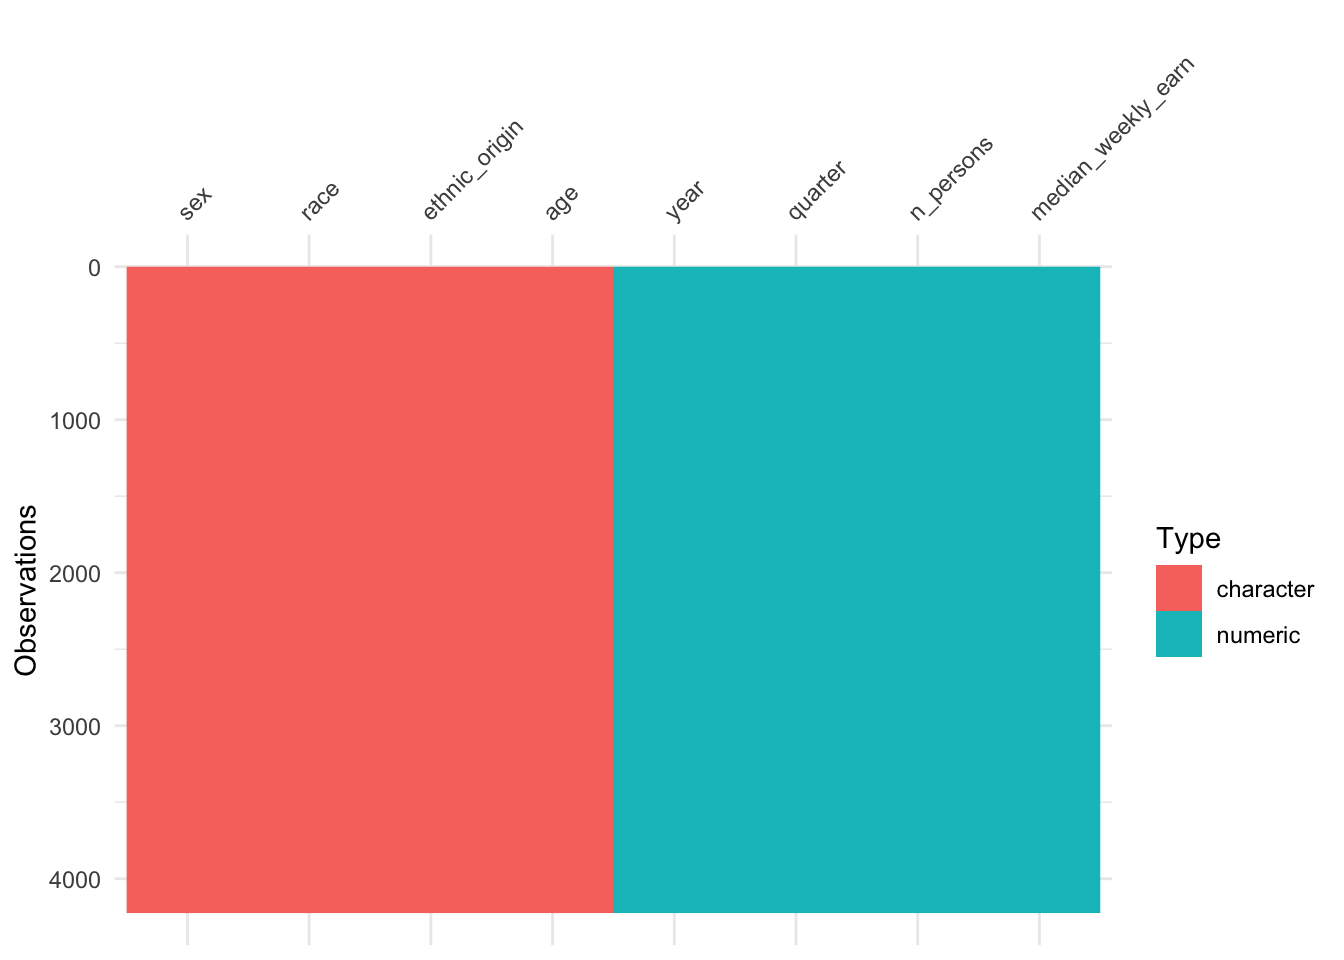
\includegraphics{earning_dataset_files/figure-latex/unnamed-chunk-1-1.pdf}

\begin{Shaded}
\begin{Highlighting}[]
\KeywordTok{vis_miss}\NormalTok{(earn)}
\end{Highlighting}
\end{Shaded}

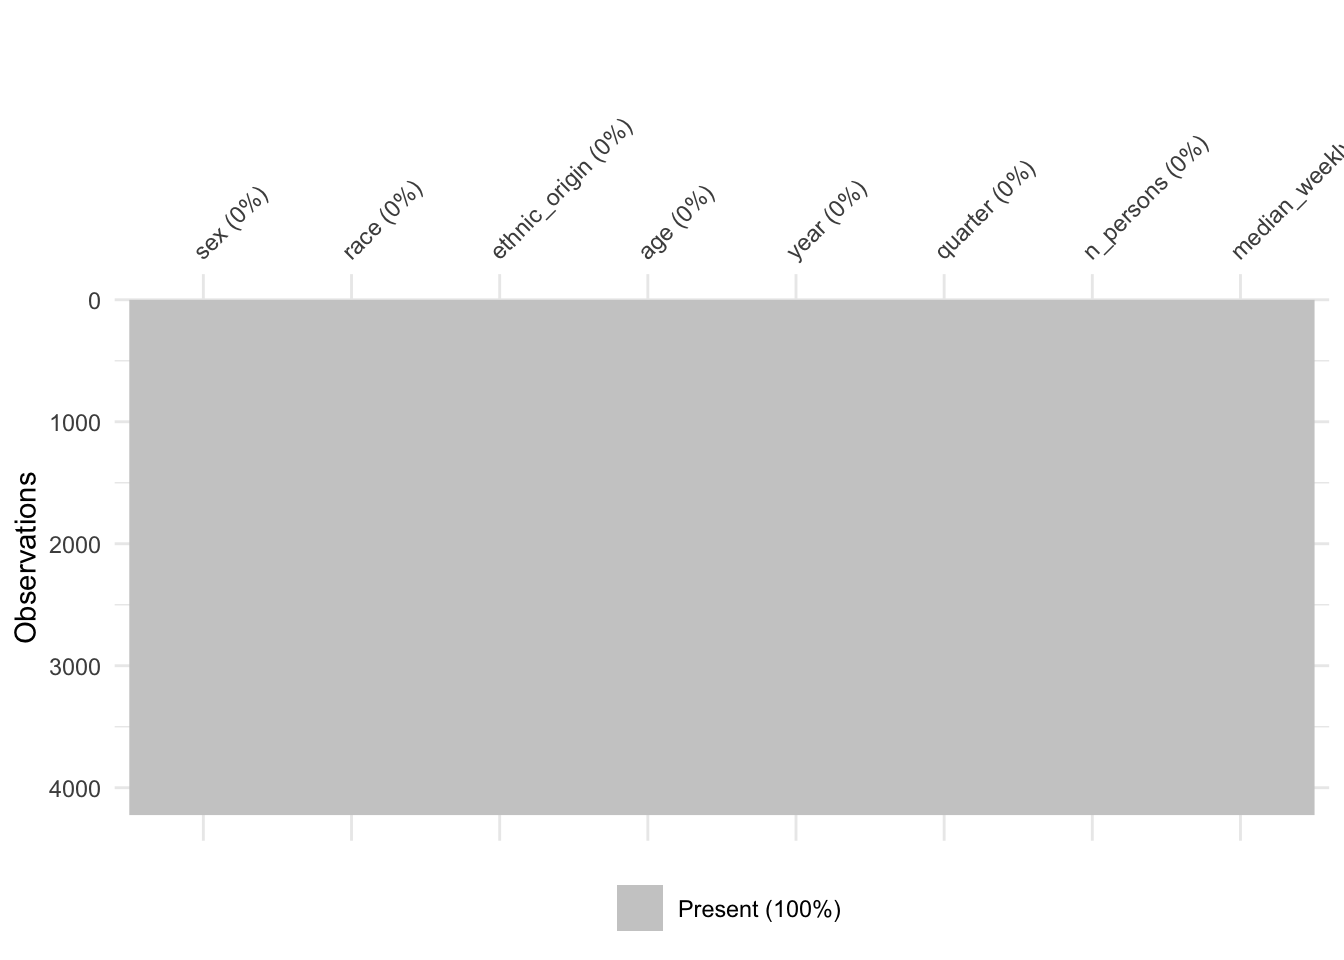
\includegraphics{earning_dataset_files/figure-latex/unnamed-chunk-1-2.pdf}

Sex and Race always seem important when we are talking about earnings!
So let's start with exploring that.

\begin{Shaded}
\begin{Highlighting}[]
\NormalTok{earn }\OperatorTok
\StringTok{  }\KeywordTok{ggplot}\NormalTok{(}\KeywordTok{aes}\NormalTok{(}
    \DataTypeTok{x =} \KeywordTok{as.character}\NormalTok{(year),}
    \DataTypeTok{y =}\NormalTok{ median_weekly_earn,}
    \DataTypeTok{colour =}\NormalTok{ sex}
\NormalTok{  )) }\OperatorTok{+}
\StringTok{  }\KeywordTok{geom_boxplot}\NormalTok{()}
\end{Highlighting}
\end{Shaded}

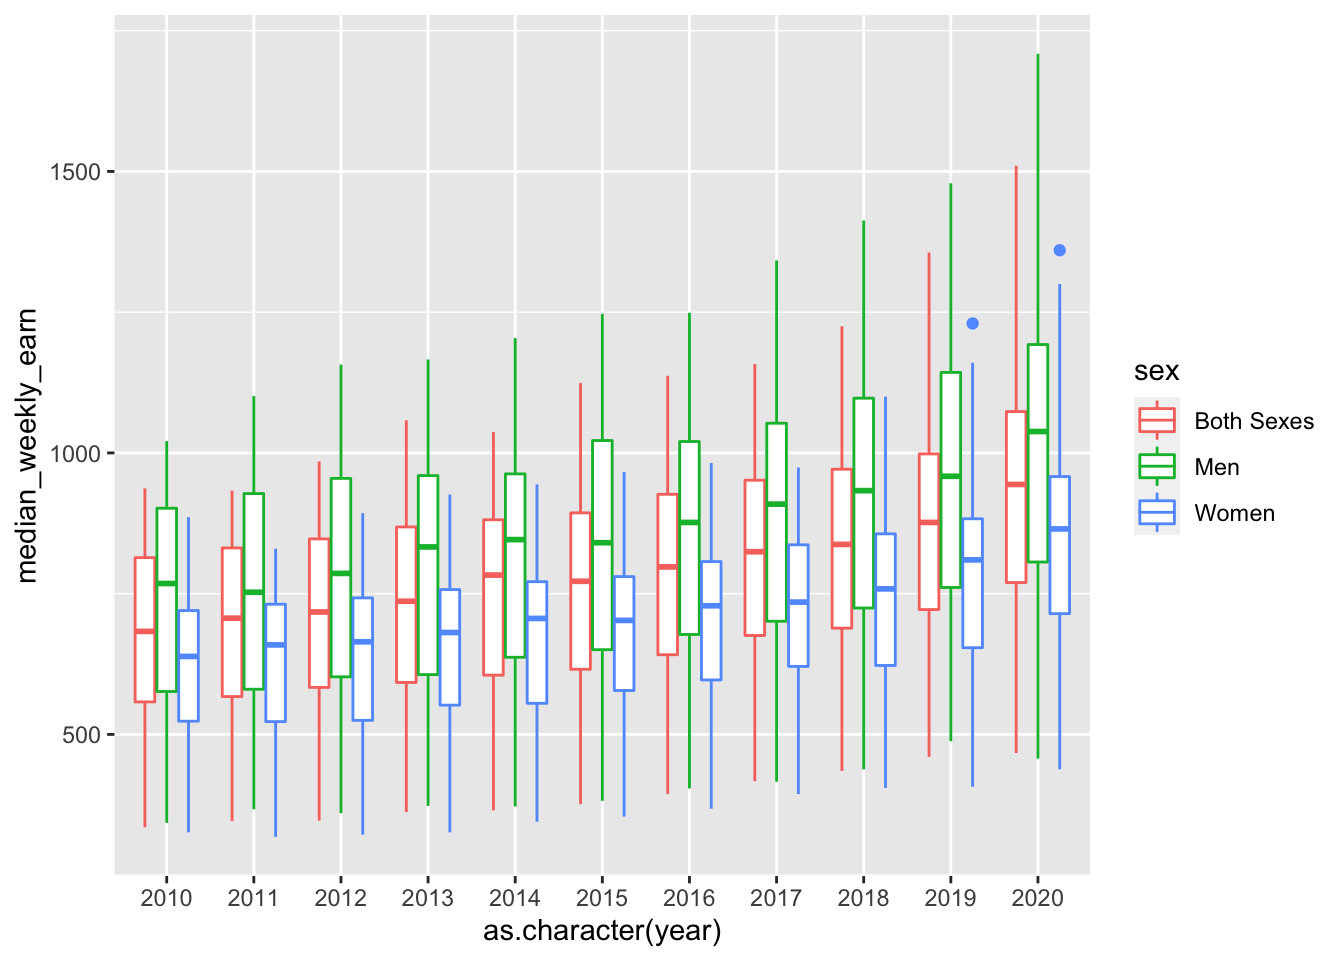
\includegraphics{earning_dataset_files/figure-latex/unnamed-chunk-2-1.pdf}

It seems like females and males both have higher weekly earning over
years and females have had lower weekly income than males consistently
over years. Further, the variability is more and increasing for men at a
higher rate than female implying a more wealth gap over years. But is
the same for all races? Let us see how are the gender pay gaps for
different races?

\begin{Shaded}
\begin{Highlighting}[]
\NormalTok{earn }\OperatorTok
\StringTok{  }\KeywordTok{filter}\NormalTok{(sex }\OperatorTok{!=}\StringTok{ "Both Sexes"}\NormalTok{) }\OperatorTok
\StringTok{  }\KeywordTok{ggplot}\NormalTok{(}\KeywordTok{aes}\NormalTok{(}\DataTypeTok{x =} \KeywordTok{as.character}\NormalTok{(year), }\DataTypeTok{y =}\NormalTok{ median_weekly_earn, }\DataTypeTok{colour =}\NormalTok{ sex, }\DataTypeTok{group =}\NormalTok{ sex)) }\OperatorTok{+}
\StringTok{  }\KeywordTok{stat_summary}\NormalTok{(}\DataTypeTok{fun =}\NormalTok{ median, }\DataTypeTok{geom =} \StringTok{"line"}\NormalTok{) }\OperatorTok{+}
\StringTok{  }\KeywordTok{facet_wrap}\NormalTok{(}\OperatorTok{~}\NormalTok{race) }\OperatorTok{+}
\StringTok{  }\KeywordTok{scale_color_brewer}\NormalTok{(}\DataTypeTok{palette =} \StringTok{"Dark2"}\NormalTok{)}
\end{Highlighting}
\end{Shaded}

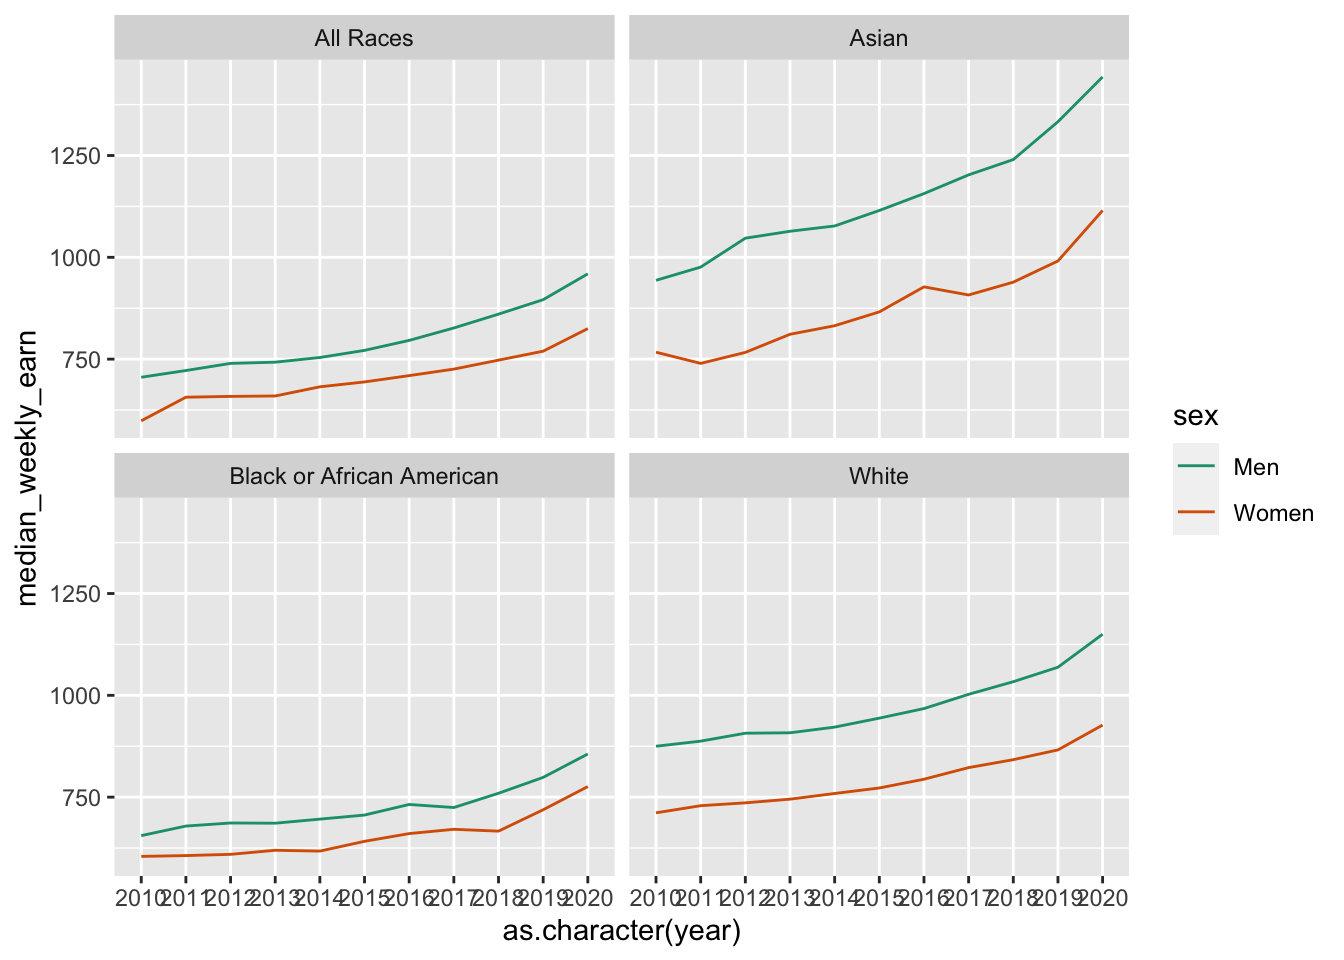
\includegraphics{earning_dataset_files/figure-latex/unnamed-chunk-3-1.pdf}

It looks like, for whites, gender gap has been almost constant over
time. Also, for African American people, gender gap is the lowest and
for Asian it is the highest. Teh gender gap looks different for
different races. What is the \% gap compared to female's earning for
each races and which race has the highest difference over years?

\begin{Shaded}
\begin{Highlighting}[]
\NormalTok{earn_tbl <-}\StringTok{ }\NormalTok{earn }\OperatorTok
\StringTok{  }\KeywordTok{ungroup}\NormalTok{() }\OperatorTok
\StringTok{  }\KeywordTok{filter}\NormalTok{(sex }\OperatorTok{!=}\StringTok{ "Both Sexes"}\NormalTok{) }\OperatorTok
\StringTok{  }\KeywordTok{group_by}\NormalTok{(year, sex, race) }\OperatorTok
\StringTok{  }\KeywordTok{mutate}\NormalTok{(}\DataTypeTok{median_earn =} \KeywordTok{median}\NormalTok{(median_weekly_earn)) }\OperatorTok
\StringTok{  }\KeywordTok{select}\NormalTok{(sex, year, median_earn, race) }\OperatorTok
\StringTok{  }\KeywordTok{unique}\NormalTok{() }\OperatorTok
\StringTok{  }\KeywordTok{pivot_wider}\NormalTok{(}
    \DataTypeTok{names_from =}\NormalTok{ sex,}
    \DataTypeTok{values_from =}\NormalTok{ median_earn}
\NormalTok{  ) }\OperatorTok
\StringTok{  }\KeywordTok{mutate}\NormalTok{(}\DataTypeTok{diff =}\NormalTok{ (Men }\OperatorTok{-}\StringTok{ }\NormalTok{Women) }\OperatorTok{*}\StringTok{ }\DecValTok{100} \OperatorTok{/}\StringTok{ }\NormalTok{Women)}


\NormalTok{earn_tbl }\OperatorTok
\StringTok{  }\KeywordTok{ggplot}\NormalTok{() }\OperatorTok{+}
\StringTok{  }\KeywordTok{geom_line}\NormalTok{(}\KeywordTok{aes}\NormalTok{(}\DataTypeTok{x =}\NormalTok{ year, }\DataTypeTok{y =}\NormalTok{ diff, }\DataTypeTok{color =}\NormalTok{ race)) }\OperatorTok{+}
\StringTok{  }\KeywordTok{scale_x_continuous}\NormalTok{(}\DataTypeTok{breaks =} \KeywordTok{seq}\NormalTok{(}\DecValTok{2010}\NormalTok{, }\DecValTok{2020}\NormalTok{, }\DecValTok{1}\NormalTok{)) }\OperatorTok{+}
\StringTok{  }\KeywordTok{ylab}\NormalTok{(}\StringTok{"% gender gap"}\NormalTok{) }\OperatorTok{+}
\StringTok{  }\KeywordTok{scale_color_viridis}\NormalTok{(}\DataTypeTok{discrete =} \OtherTok{TRUE}\NormalTok{) }\OperatorTok{+}
\StringTok{  }\KeywordTok{theme_void}\NormalTok{() }\OperatorTok{+}
\StringTok{  }\KeywordTok{theme_dark}\NormalTok{() }\OperatorTok{+}
\StringTok{  }\KeywordTok{theme}\NormalTok{(}\DataTypeTok{legend.position =} \StringTok{"bottom"}\NormalTok{)}
\end{Highlighting}
\end{Shaded}

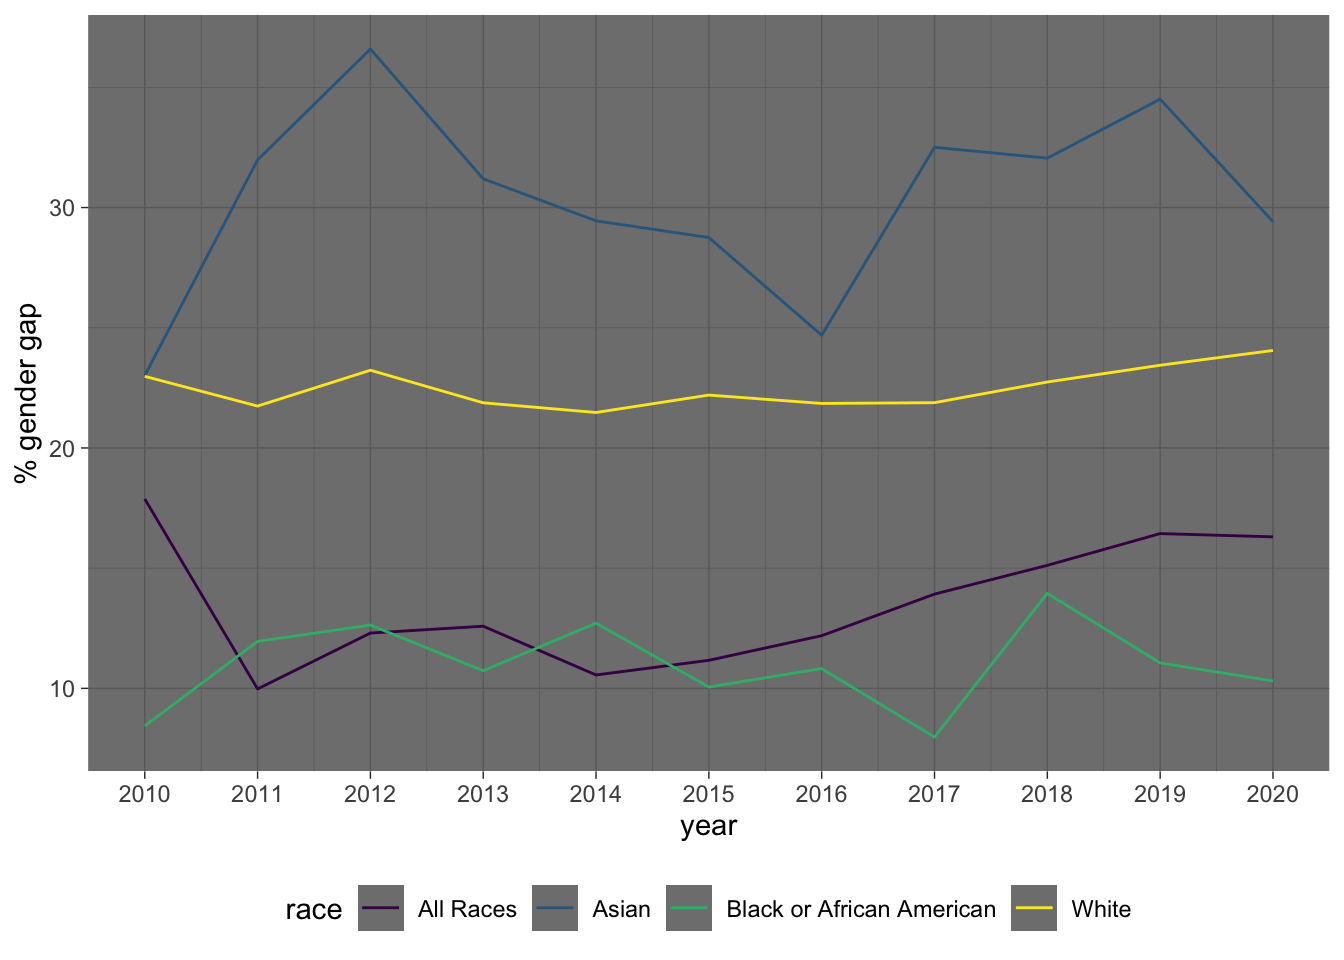
\includegraphics{earning_dataset_files/figure-latex/unnamed-chunk-4-1.pdf}

For whites, the percentage gender gap has been constantly staying at
aroiund 20\% over years. For African American it is increasing from 10\%
to 15\% from 2014 to 2020. For Asians, this pattern is just the opposite
where the percentage gender gap is decreasing from 2012 to 2016 and then
increasing after 2016. This could be a result of the political situation
back in the US, when during Obama's presidential term, the gender gap
was decreasing and then again started increasing during the presidency
of Trump.

On further discussions with other teams, we were interested to explore
if the gender gap changes across quarters and age. It looks like for all
quarters, more or less, the story has been the same. But for age, with
increasing age, the gap between male and female pay just gets worse and
the variability is the most for the age group 16-24 and 25-54.

\begin{Shaded}
\begin{Highlighting}[]
\NormalTok{earn }\OperatorTok\StringTok{ }
\StringTok{  }\KeywordTok{filter}\NormalTok{(sex }\OperatorTok{!=}\StringTok{ "Both Sexes"}\NormalTok{) }\OperatorTok
\StringTok{  }\KeywordTok{ggplot}\NormalTok{(}\KeywordTok{aes}\NormalTok{(}
    \DataTypeTok{x =} \KeywordTok{as.character}\NormalTok{(year),}
    \DataTypeTok{y =}\NormalTok{ median_weekly_earn,}
    \DataTypeTok{fill =}\NormalTok{ sex}
\NormalTok{  )) }\OperatorTok{+}
\StringTok{  }\KeywordTok{geom_violin}\NormalTok{() }\OperatorTok{+}
\StringTok{  }\KeywordTok{facet_wrap}\NormalTok{(}\OperatorTok{~}\NormalTok{quarter) }\OperatorTok{+}
\StringTok{  }\KeywordTok{scale_fill_viridis}\NormalTok{(}\DataTypeTok{discrete =} \OtherTok{TRUE}\NormalTok{, }\DataTypeTok{direction =} \DecValTok{-1}\NormalTok{) }\OperatorTok{+}
\StringTok{  }\KeywordTok{theme}\NormalTok{(}\DataTypeTok{axis.text.x =} \KeywordTok{element_text}\NormalTok{(}\DataTypeTok{angle =} \DecValTok{90}\NormalTok{, }\DataTypeTok{vjust =} \FloatTok{0.5}\NormalTok{, }\DataTypeTok{hjust=}\DecValTok{1}\NormalTok{))}
\end{Highlighting}
\end{Shaded}

\includegraphics{earning_dataset_files/figure-latex/unnamed-chunk-5-1.pdf}

\begin{Shaded}
\begin{Highlighting}[]
\NormalTok{earn }\OperatorTok
\StringTok{  }\KeywordTok{filter}\NormalTok{(}\OperatorTok{!}\NormalTok{(age }\OperatorTok\StringTok{ }
\StringTok{           }\KeywordTok{c}\NormalTok{(}\StringTok{"16 years and over"}\NormalTok{, }
             \StringTok{"25 years and over"}\NormalTok{,}
             \StringTok{"55 years and over"}\NormalTok{,}
             \StringTok{"65 years and over"}\NormalTok{))) }\OperatorTok\StringTok{ }
\StringTok{  }\KeywordTok{filter}\NormalTok{(sex }\OperatorTok{!=}\StringTok{ "Both Sexes"}\NormalTok{) }\OperatorTok
\StringTok{  }\KeywordTok{ggplot}\NormalTok{(}\KeywordTok{aes}\NormalTok{(}
    \DataTypeTok{x =} \KeywordTok{as.character}\NormalTok{(year),}
    \DataTypeTok{y =}\NormalTok{ median_weekly_earn,}
    \DataTypeTok{colour =}\NormalTok{ sex}
\NormalTok{  )) }\OperatorTok{+}
\StringTok{  }\KeywordTok{geom_boxplot}\NormalTok{() }\OperatorTok{+}
\StringTok{  }\KeywordTok{facet_wrap}\NormalTok{(}\OperatorTok{~}\NormalTok{age) }\OperatorTok{+}
\StringTok{  }\KeywordTok{scale_color_brewer}\NormalTok{(}\DataTypeTok{palette =} \StringTok{"RdPu"}\NormalTok{) }\OperatorTok{+}\StringTok{ }
\StringTok{  }\KeywordTok{theme_dark}\NormalTok{() }\OperatorTok{+}\StringTok{ }
\StringTok{  }\KeywordTok{theme}\NormalTok{(}\DataTypeTok{axis.text.x =} \KeywordTok{element_text}\NormalTok{(}\DataTypeTok{angle =} \DecValTok{90}\NormalTok{, }\DataTypeTok{vjust =} \FloatTok{0.5}\NormalTok{, }\DataTypeTok{hjust=}\DecValTok{1}\NormalTok{))}
\end{Highlighting}
\end{Shaded}

\includegraphics{earning_dataset_files/figure-latex/unnamed-chunk-6-1.pdf}

\end{document}
